% !TEX program = pdflatex
\documentclass[aspectratio=169]{beamer}

% THEME (using metropolis for a modern, eye-catching look; seahorse colors for contrast)
\usetheme{metropolis}
\usecolortheme{seahorse}
\usepackage{graphicx}
\usepackage{tikz}
\usepackage{xcolor}
\definecolor{DarkGreen}{RGB}{0,100,0} 
\usetikzlibrary{shapes,arrows,}
\setbeamertemplate{navigation symbols}{}
\setbeamertemplate{footline}[frame number]

\usepackage[utf8]{inputenc}
\usepackage{graphicx}
\usepackage{booktabs}
\usepackage{hyperref}
\usepackage{tikz} %  Added for potential diagrams and enhanced visuals

% Custom styles for eye-catching elements
\definecolor{highlightcolor}{RGB}{0, 128, 255} % Bright blue for highlights
\newcommand{\highlight}[1]{\textcolor{highlightcolor}{\textbf{#1}}}
\newcommand{\alertitem}[1]{\item \alert{#1}} % For emphasized bullet points

% Placeholder macro for topology input
\newcommand{\topologyplaceholder}{\texttt{[Insert Topology Here, e.g., Star, Mesh, Hierarchical]}}

% Touhid
\usepackage{array,booktabs}
\usepackage[table]{xcolor}   % rowcolors + colors in tables
\usepackage{colortbl}        % \arrayrulecolor
\usepackage{tikz}
\usetikzlibrary{arrows.meta,positioning,shadows.blur,fit,calc}

% Colors (define once)
\definecolor{pri}{RGB}{0,120,212}   % primary blue
\definecolor{acc}{RGB}{3,166,120}   % accent green
\definecolor{mut}{RGB}{120,120,120} % muted gray

% Beamer theme tweaks
\setbeamertemplate{navigation symbols}{}
\setbeamercolor{title}{fg=pri}
\setbeamercolor{frametitle}{fg=pri}
\setbeamerfont{frametitle}{series=\bfseries}

% Custom alert block styling for metropolis theme
\setbeamercolor{block title alerted}{bg=red!85!black,fg=white}
\setbeamercolor{block body alerted}{bg=red!10,fg=black}
\setbeamerfont{block title alerted}{series=\bfseries}

% --- TikZ styles ---
\tikzset{
  router/.style={circle,draw=black,fill=white,very thick,minimum size=9mm,drop shadow},
  link/.style={-Latex,ultra thick,draw=pri!80},  % thicker, blue-toned
  linkmut/.style={-Latex,thick,draw=mut},
  linkdash/.style={-Latex,ultra thick,dashed,draw=acc},
  badge/.style={rectangle,rounded corners=2pt,fill=pri!10,draw=pri,inner sep=2pt,font=\scriptsize},
  % Your upgraded flowstep style (with subtle gradient + shadow)
  flowstep/.style={
    rectangle,rounded corners=4pt,
    draw=black,very thick,
    top color=white,bottom color=pri!5,
    minimum height=8mm,inner sep=6pt, % a bit more padding
    drop shadow
  },
  good/.style={circle,draw=acc,very thick,minimum size=5mm},
  bad/.style={circle,draw=pri,very thick,minimum size=5mm},
}


% ---------- Meta ----------


% ---------- DOCUMENT ----------
\begin{document}

% ---------- Title ----------
%---------------------------------------------
% Title Page — RUET Style
%---------------------------------------------
\begin{frame}
\centering
\vspace{-0.15cm}

\includegraphics[width=2cm]{ruet-logo.png}\\[3pt]

{\small\textbf{Rajshahi University of Engineering \& Technology}}\\[2pt]
\rule{0.5\linewidth}{0.3pt}\\[6pt]
{\footnotesize\textcolor{highlightcolor}{\textbf{Understanding Static and Dynamic Routing (RIP) in Campus Networks}}}\\[2pt]
{\footnotesize\textit{Ethical, Societal, and Environmental Considerations}}\\[4pt]

{\small\textbf{CSE 4104: Computer Networks Sessional}}\\[1pt]
{\small\textbf{Section A}}\\[2pt]

{\footnotesize
Md Touhidul Islam (2003051)\\
Mustain Ahmed (2003052)\\
Md. Tanvir Kabir Akon (2003053)\\
Nur E Mahbubul Islam (2003054)\\
Eazdan Mostafa Rafin (2003055)}
\end{frame}

% ---------- Part-1 Section: Introduction (Rafin) ----------
\section{Introduction}

% Slide 1 — Scope of the Introduction
\begin{frame}{Introduction}
\begin{itemize}
    \item A \textbf{Campus Network} connects multiple departments such as Administration, EEE, and CSE within the same organization.
    \item The network includes several layers:
    \begin{itemize}
        \item \textbf{Core Layer:} Main backbone connecting internal and external networks.
        \item \textbf{Distribution Layer:} Handles inter-VLAN routing and policy enforcement.
        \item \textbf{Access Layer:} Provides connectivity for end devices such as PCs, printers, and servers.
    \end{itemize}
    \item This topology ensures efficient communication, scalability, and secure data flow between departments.
\end{itemize}
\end{frame}
%----------Topology Slide (optional)----------
\begin{frame}{Campus Network Topology}
\begin{figure}[H]
    \centering
    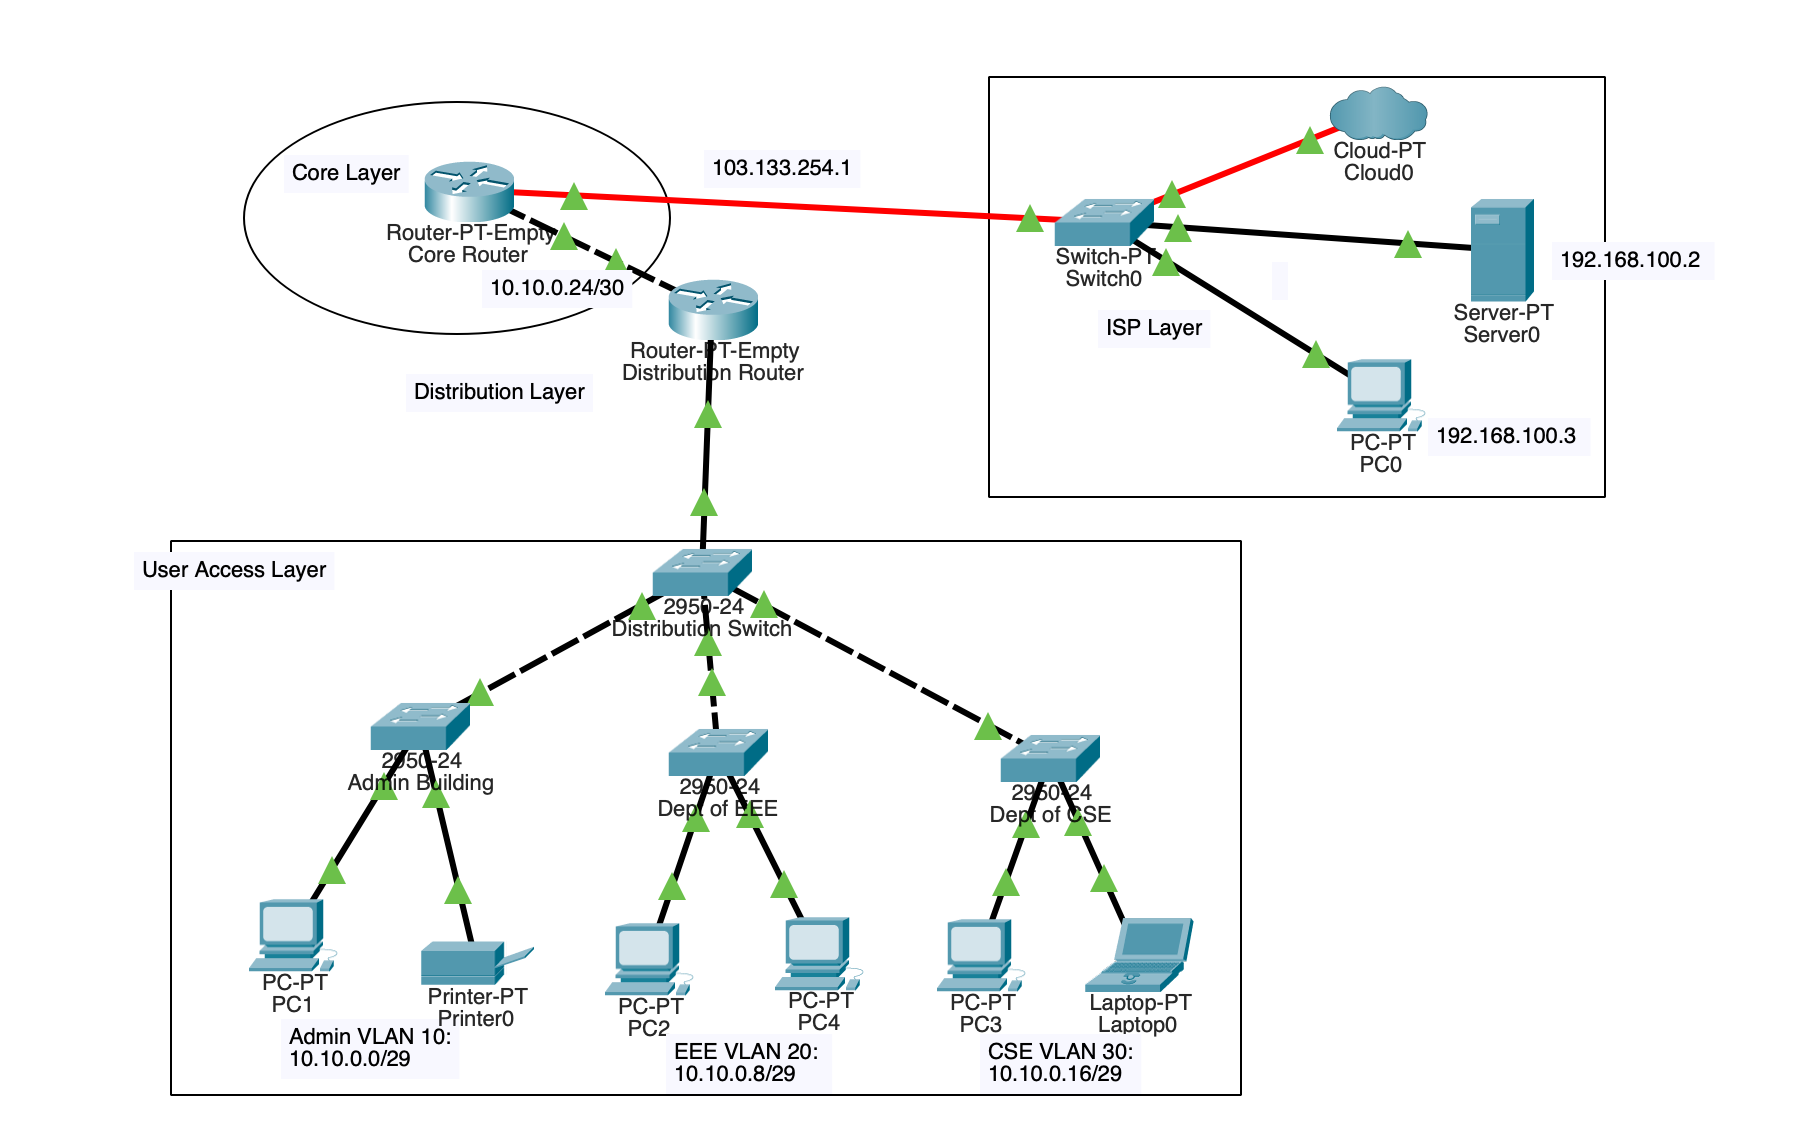
\includegraphics[width=0.75\linewidth]{topology.png}
    \caption{Campus Network Topology showing Core, Distribution, and Access Layers}
\end{figure}
\end{frame}
%---------------------------------------------
\begin{frame}{Static Routing Overview}
\begin{itemize}
    \item \textbf{Static Routing:} Manually configured routes that define fixed paths for data packets.
    \item Ensures reliable and predictable routing within small to medium networks.
    \item Used between routers in the Core and Distribution layers.
    \item Types of static routes:
    \begin{itemize}
        \item \textbf{Standard Static Route:} For specific internal subnets.
        \item \textbf{Default Route:} Used when no other route matches (typically toward ISP).
        \item \textbf{Floating Static Route:} Acts as a backup route with a higher administrative distance.
    \end{itemize}
\end{itemize}
\end{frame}

%---------------------------------------------
\begin{frame}{Static Routing in Campus Network}
\begin{itemize}
    \item \textbf{Standard Static Route:} Connects Core to internal VLANs through the Distribution router.
    \begin{itemize}
        \item Example: \texttt{ip route 10.10.0.0 255.255.255.224 10.10.0.26}
    \end{itemize}
    \item \textbf{Default Route:} Forwards all unknown traffic toward ISP.
    \begin{itemize}
        \item Example: \texttt{ip route 0.0.0.0 0.0.0.0 103.133.254.2}
    \end{itemize}
    \item \textbf{Floating Static Route:} Backup path activated if main link fails.
    \begin{itemize}
        \item Example: \texttt{ip route 0.0.0.0 0.0.0.0 10.10.0.26 250}
    \end{itemize}
\end{itemize}
\end{frame}

%---------------------------------------------
\begin{frame}{Dynamic Routing (RIP)}
\begin{itemize}
    \item \textbf{Dynamic Routing Protocols} allow routers to automatically share and update routing information.
    \item In this network, \textbf{RIP (Routing Information Protocol)} can be used:
    \begin{itemize}
        \item Exchanges routes based on hop count metric.
        \item Simplifies configuration and adapts to topology changes.
    \end{itemize}
    \item Combining \textbf{Static Routing} (for control) and \textbf{RIP} (for flexibility) improves network resilience.
\end{itemize}
\end{frame}
% ----------part-2,3 Akon----------






%----------part-4 Section: Environmental Impact (Mustain)----------
\begin{frame}{Environmental Impact of Networking Devices}
    \framesubtitle{Energy Consumption Factors}
    
    Networking devices contribute significantly to energy usage through:
    \begin{itemize}
        \item \textbf{CPU Processing}: Routing calculations and protocol operations
        \item \textbf{Memory Usage}: Maintaining routing tables and network state
        \item \textbf{Network Traffic}: Packet forwarding and processing load
        \item \textbf{Protocol Overhead}: Update frequency and message processing
    \end{itemize}
 
    \begin{alertblock}{Environmental Concern}
        \vspace{0.1cm}
        Higher routing activity $\rightarrow$ More CPU usage $\rightarrow$ Higher energy consumption $\rightarrow$ Greater environmental impact
    \end{alertblock}
\end{frame}

% --- Frame 3: Comparative Analysis ---
\begin{frame}{Static vs Dynamic Routing: Environmental Comparison}
    \small
    \begin{table}
    \centering
    \begin{tabular}{|p{2.2cm}|p{2.8cm}|p{3.2cm}|}
    \hline
    \textbf{Parameter} & \textbf{Static Routing} & \textbf{RIP Dynamic Routing} \\ \hline
    Configuration & Manual, simple & Automatic, complex \\ \hline
    CPU Usage & \textcolor{DarkGreen}{Low} & \textcolor{red}{High} \\ \hline
    Memory Requirements & \textcolor{DarkGreen}{Minimal} & \textcolor{red}{Significant} \\ \hline
    Update Frequency & \textcolor{DarkGreen}{None} & \textcolor{red}{Every 30 seconds} \\ \hline
    Network Overhead & \textcolor{DarkGreen}{Zero} & \textcolor{red}{Regular updates} \\ \hline
    Energy Consumption & \textcolor{DarkGreen}{Low} & \textcolor{red}{High} \\ \hline
    Environmental Impact & \textcolor{DarkGreen}{Less} & \textcolor{red}{High} \\ \hline
    \end{tabular}
    \end{table}
\end{frame}

% --- Frame 4: Energy-Efficient Practices ---
\begin{frame}{Energy-Efficient Routing: Best Practices}
    
    \textbf{Protocol Optimization}
    \begin{itemize}
        \item \textbf{Adjust Update Intervals}: Increase RIP timers from 30 to 60+ seconds
        \item \textbf{Use Passive Interfaces}: Prevent unnecessary routing updates
        \item \textbf{Implement Route Summarization}: Reduce routing table size
        \item \textbf{Choose Efficient Protocols}: Consider OSPF or EIGRP with better scaling
    \end{itemize}
    
    \vspace{0.4cm}
    
    \textbf{Hardware Management}
    \begin{itemize}
        \item \textbf{Port Management}: Disable unused ports and interfaces
        \item \textbf{Link Aggregation}: Consolidate traffic and power down idle links
        \item \textbf{Power Scheduling}: Implement off-peak shutdown procedures
        \item \textbf{Energy-Aware Hardware}: Use devices with power management features
    \end{itemize}
\end{frame}

%----------Part-5 Section: Best Practices (Touhid)----------
\section{Best Practices}
\begin{frame}{Static vs Floating Static vs RIP}
\small

\begin{table}
\centering
\rowcolors{2}{pri!10}{white}
\arrayrulecolor{pri!60}
\begin{tabular}{@{}>{\bfseries\arraybackslash}m{3.2cm}
                >{\centering\arraybackslash}m{3.0cm}
                >{\centering\arraybackslash}m{3.0cm}
                >{\centering\arraybackslash}m{4.2cm}@{}}
\toprule
\rowcolor{pri!25}\bfseries Type & \bfseries Reliability & \bfseries Ease of Setup & \bfseries Ethical Considerations \\
\midrule
Static & High (manual) & Easy (small nets) & Keep routes updated; avoid stale paths \\
\textbf{Floating Static} & High (with backup) & Moderate (priorities) & Don’t abuse metrics to prefer unfair paths \\
\textbf{RIP (Dynamic)} & Adaptive (changes) & Simple, scalable & Secure updates; prevent false adverts \\
\bottomrule
\end{tabular}
\rowcolors{2}{white}{white}
\end{table}

\vspace{0.4cm}
\centering
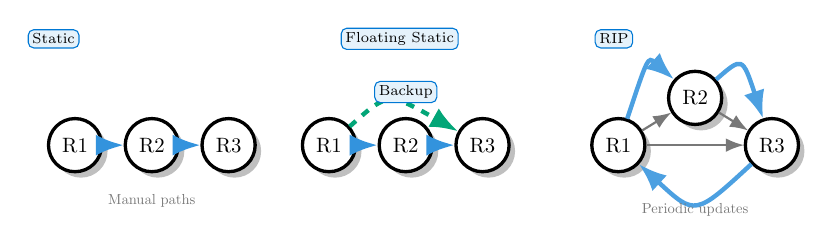
\begin{tikzpicture}[scale=0.75, every node/.style={transform shape}]
% Labels
\node[badge,anchor=west] (b1) at (-5.8,1.8) {Static};
\node[badge,anchor=west] (b2) at (-0.5,1.8) {Floating Static};
\node[badge,anchor=west] (b3) at (3.8,1.8) {RIP};

% --- Static cluster ---
\node[router] (S1) at (-5,0){R1};
\node[router] (S2) at (-3.7,0){R2};
\node[router] (S3) at (-2.4,0){R3};
\draw[link] (S1) -- (S2);
\draw[link] (S2) -- (S3);
\node[align=center,mut,scale=0.7] at (-3.7,-0.95) {Manual paths};

% --- Floating Static cluster ---
\node[router] (F1) at (-0.7,0){R1};
\node[router] (F2) at (0.6,0){R2};
\node[router] (F3) at (1.9,0){R3};
\draw[link] (F1) -- (F2);
\draw[link] (F2) -- (F3);
% backup diagonal
\draw[linkdash] (F1) .. controls (0.3,0.9) .. (F3);
\node[badge] at (0.6,0.9) {Backup};

% --- RIP cluster ---
\node[router] (D1) at (4.2,0){R1};
\node[router] (D2) at (5.5,0.8){R2};
\node[router] (D3) at (6.8,0){R3};
\draw[linkmut] (D1) -- (D2);
\draw[linkmut] (D2) -- (D3);
\draw[linkmut] (D1) -- (D3);
% dynamic arrows
\draw[-Latex,ultra thick,draw=pri!70] (D1) .. controls (4.7,1.5) .. (D2);
\draw[-Latex,ultra thick,draw=pri!70] (D2) .. controls (6.3,1.5) .. (D3);
\draw[-Latex,ultra thick,draw=pri!70] (D3) .. controls (5.5,-1.2) .. (D1);
\node[align=center,mut,scale=0.7] at (5.5,-1.1) {Periodic updates};
\end{tikzpicture}
\end{frame}

% ------------------- Slide 2 -------------------
\begin{frame}{Best Practices \& Outage Prevention}
\small
\begin{columns}[T,onlytextwidth]

% Left: flow with subtext anchors
\begin{column}{0.55\textwidth}
\centering
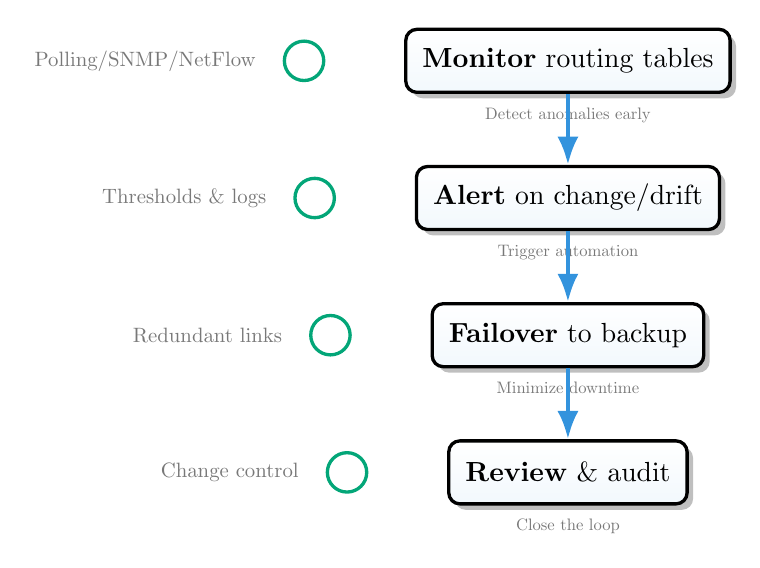
\begin{tikzpicture}[node distance=9mm and 10mm]
\node[flowstep] (m)  {\textbf{Monitor} routing tables};
\node[mut,scale=0.6,below=1mm of m] {Detect anomalies early};

\node[flowstep,below=of m] (a) {\textbf{Alert} on change/drift};
\node[mut,scale=0.6,below=1mm of a] {Trigger automation};

\node[flowstep,below=of a] (f) {\textbf{Failover} to backup};
\node[mut,scale=0.6,below=1mm of f] {Minimize downtime};

\node[flowstep,below=of f] (r) {\textbf{Review} \& audit};
\node[mut,scale=0.6,below=1mm of r] {Close the loop};

% Flow arrows
\draw[link] (m) -- (a);
\draw[link] (a) -- (f);
\draw[link] (f) -- (r);

% side notes (slightly more breathing room)
\node[good,left=10mm of m] (g1) {};
\node[align=right,mut,scale=0.75,anchor=east] at ($(g1.west)+(-0.25,0)$) {Polling/SNMP/NetFlow};

\node[good,left=10mm of a] (g2) {};
\node[align=right,mut,scale=0.75,anchor=east] at ($(g2.west)+(-0.25,0)$) {Thresholds \& logs};

\node[good,left=10mm of f] (g3) {};
\node[align=right,mut,scale=0.75,anchor=east] at ($(g3.west)+(-0.25,0)$) {Redundant links};

\node[good,left=10mm of r] (g4) {};
\node[align=right,mut,scale=0.75,anchor=east] at ($(g4.west)+(-0.25,0)$) {Change control};
\end{tikzpicture}
\end{column}

% Right: topology + concise takeaways
\begin{column}{0.45\textwidth}
\centering
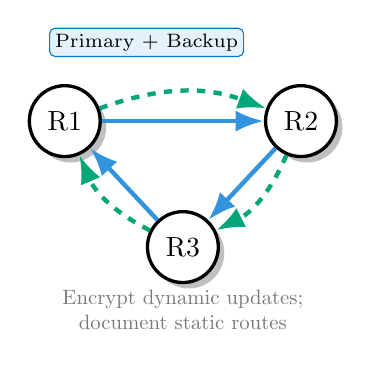
\begin{tikzpicture}
% Redundant mini-topology (primary + backup)
\node[router] (A) at (0,0){R1};
\node[router] (B) at (3,0){R2};
\node[router] (C) at (1.5,-1.6){R3};

\draw[link]    (A) -- (B);
\draw[link]    (B) -- (C);
\draw[link]    (C) -- (A);
% backup links (dashed)
\draw[linkdash] (A) to[bend left=20] (B);
\draw[linkdash] (B) to[bend left=20] (C);
\draw[linkdash] (C) to[bend left=20] (A);

\node[badge,anchor=west] at (-0.2,1.0) {Primary + Backup};
\node[align=center,mut,scale=0.75] at (1.5,-2.4) {Encrypt dynamic updates;\\document static routes};
\end{tikzpicture}

\vspace{2mm}
\footnotesize
\begin{tabular}{@{}>{\bfseries}l l@{}}
Static:   & Update on change \\
Floating: & Test failover \\
RIP:      & Authenticate updates \\
\end{tabular}
\end{column}

\end{columns}
\end{frame}

%------Conclusion Slide------
\section{Conclusion}
\begin{frame}{Summary of Key Points}
\begin{itemize}
    \item \textbf{Ethical:} Fair access, secure routing, documented changes.
    \vspace{4pt}
    \item \textbf{Societal:} Reliable connectivity supports learning and management.
    \vspace{4pt}
    \item \textbf{Performance:} Three-layer design ensures scalability and efficiency.
    \vspace{4pt}
    \item \textbf{Integration:} Static + RIP + Floating Static for stable hybrid routing.
\end{itemize}
\end{frame}

\begin{frame}{Recommendations for Simple, Reliable, and Fair Routing}
\begin{itemize}
    \item \textbf{Adopt Hierarchical Design:} Use Core, Distribution, and Access layers for easier control and scalability.
    \vspace{6pt}
    \item \textbf{Prefer Static Routes:} Keep internal routing simple and predictable.
    \vspace{6pt}
    \item \textbf{Use RIP Version 2:} Allow automatic route exchange with subnet mask support for flexible updates.
    \vspace{6pt}
    \item \textbf{Add Floating Static Routes:} Maintain backup links for failover and reliability.
    \vspace{6pt}
    \item \textbf{Ensure Fair Access:} Apply VLAN segmentation for secure and balanced traffic flow.
    \vspace{6pt}
    \item \textbf{Monitor and Document:} Keep routing tables and configurations updated for transparency.
\end{itemize}
\end{frame}
\begin{frame}
\centering
\Huge \textbf{Thank You!}
\end{frame}
\end{document}